\hypertarget{qnote_8cpp}{}\section{O\+L13/qnote.cpp File Reference}
\label{qnote_8cpp}\index{O\+L13/qnote.\+cpp@{O\+L13/qnote.\+cpp}}


Définitions des fonctions déclarées dans le qnotes.\+h.  


{\ttfamily \#include \char`\"{}qnote.\+h\char`\"{}}\newline
Include dependency graph for qnote.\+cpp\+:\nopagebreak
\begin{figure}[H]
\begin{center}
\leavevmode
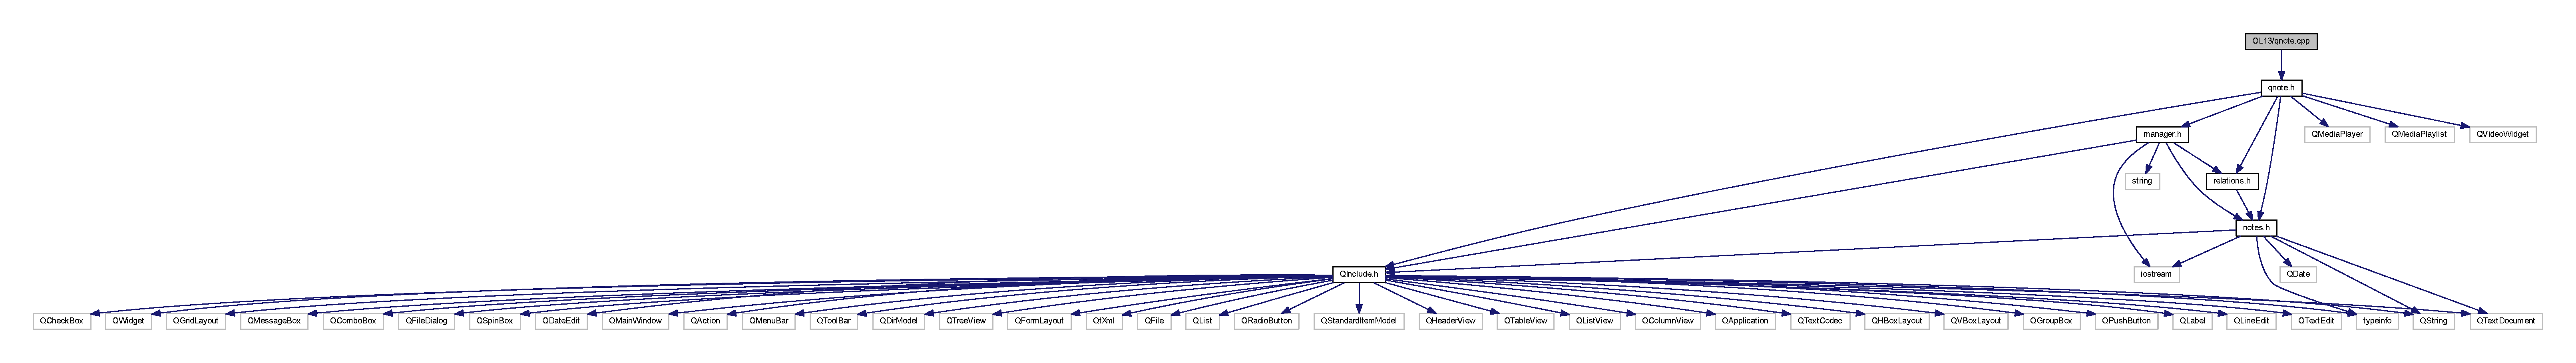
\includegraphics[width=350pt]{qnote_8cpp__incl}
\end{center}
\end{figure}


\subsection{Detailed Description}
Définitions des fonctions déclarées dans le qnotes.\+h. 

\begin{DoxyAuthor}{Author}
Garnier Maxime, Naudin Louise, Pépin Hugues 
\end{DoxyAuthor}
\begin{DoxyVersion}{Version}
1.\+0 
\end{DoxyVersion}
\begin{DoxyDate}{Date}
14 Juin 2017
\end{DoxyDate}
Domaines des méthodes comprises dans ce fichier \+:
\begin{DoxyItemize}
\item Constructeur
\item Destructeur
\item Affichage
\item Sauvegarde
\item Chargement Le détail est donné dans la suite du fichier. 
\end{DoxyItemize}